\documentclass[aspectratio=169]{beamer}

\usepackage[utf8]{inputenc}
\usepackage{tikz}
\usetikzlibrary{positioning, arrows.meta}

\usefonttheme{professionalfonts}

% Theme
\usetheme{Madrid}
\definecolor{ucdgreen}{RGB}{0, 102, 51}
\definecolor{gapred}{RGB}{180, 50, 50}
\definecolor{vennblue}{RGB}{70, 130, 180}
\definecolor{vennorange}{RGB}{210, 140, 50}
\usecolortheme[named=ucdgreen]{structure}
\setbeamertemplate{navigation symbols}{}

\title[Research Studies Panel]{Research Studies Panel}
\author[Lainey Ward]{Lainey Ward}
\institute[]{}
\date{}

\begin{document}

% --------------------------------------------------
% BACKUP: Literature review scope (Venn diagram)
% --------------------------------------------------
% USE: If panel asks "how did you scope the review?"
%      or "what fields does this draw from?"
% --------------------------------------------------
\begin{frame}{Where the Literature Review Sits}

    \centering
    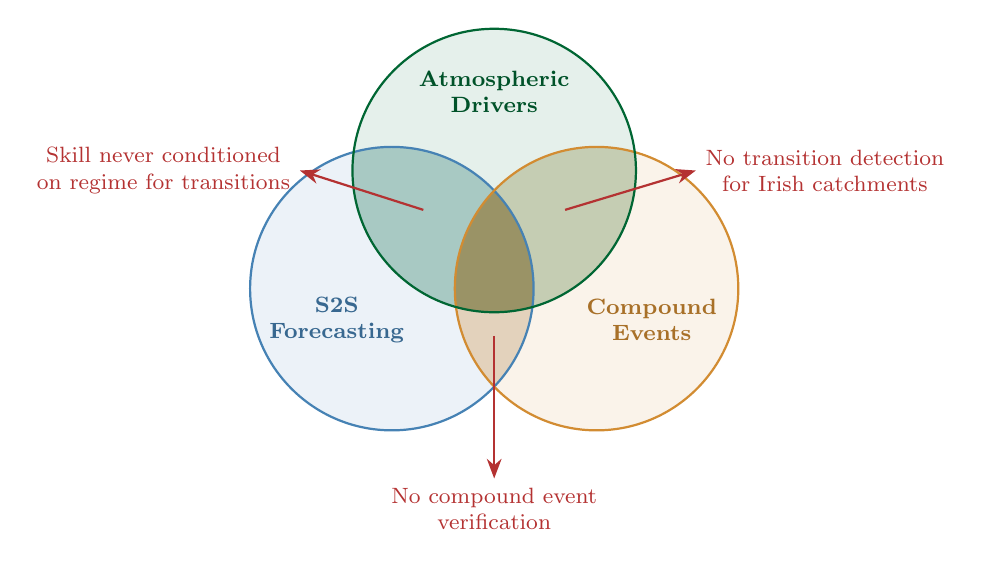
\begin{tikzpicture}
    \def\r{1.8}

    % Base circle fills
    \fill[vennblue!10] (-1.3,0) circle (\r);
    \fill[vennorange!10] ( 1.3,0) circle (\r);
    \fill[ucdgreen!10] (0,1.5) circle (\r);

    % Pairwise overlap fills
    \begin{scope}
      \clip (-1.3,0) circle (\r);
      \clip ( 1.3,0) circle (\r);
      \fill[vennblue!25!vennorange, opacity=0.3] (-3,-3) rectangle (3,3);
    \end{scope}
    \begin{scope}
      \clip (-1.3,0) circle (\r);
      \clip (0,1.5) circle (\r);
      \fill[vennblue!40!ucdgreen, opacity=0.3] (-3,-3) rectangle (3,3);
    \end{scope}
    \begin{scope}
      \clip ( 1.3,0) circle (\r);
      \clip (0,1.5) circle (\r);
      \fill[ucdgreen!40!vennorange, opacity=0.3] (-3,-3) rectangle (3,3);
    \end{scope}

    % Triple intersection fill
    \begin{scope}
      \clip (-1.3,0) circle (\r);
      \clip ( 1.3,0) circle (\r);
      \clip (0,1.5) circle (\r);
      \fill[ucdgreen!30!vennblue!30!vennorange, opacity=0.5] (-3,-3) rectangle (3,3);
    \end{scope}

    % Circle outlines
    \draw[vennblue, thick] (-1.3,0) circle (\r);
    \draw[vennorange, thick] ( 1.3,0) circle (\r);
    \draw[ucdgreen, thick] (0,1.5) circle (\r);

    % Circle labels
    \node[align=center, text=vennblue!80!black, font=\footnotesize\bfseries]
        at (-2.0,-0.4) {S2S\\Forecasting};
    \node[align=center, text=vennorange!80!black, font=\footnotesize\bfseries]
        at ( 2.0,-0.4) {Compound\\Events};
    \node[align=center, text=ucdgreen!80!black, font=\footnotesize\bfseries]
        at (0,2.5) {Atmospheric\\Drivers};

    % Pairwise gap labels — updated to match validated gaps
    % Forecast × Compound Events (bottom)
    \node[align=center, font=\footnotesize, text=gapred] (g1) at (0,-2.8)
         {No compound event\\verification};
    \draw[-{Stealth[length=2.5mm]}, thick, gapred] (0,-0.6) -- (g1.north);

    % Forecast × Drivers (upper-left)
    \node[align=center, font=\footnotesize, text=gapred] (g2) at (-4.2,1.5)
         {Skill never conditioned\\on regime for transitions};
    \draw[-{Stealth[length=2.5mm]}, thick, gapred] (-0.9,1.0) -- (g2.east);

    % Drivers × Compound Events (upper-right)
    \node[align=center, font=\footnotesize, text=gapred] (g3) at (4.2,1.5)
         {No transition detection\\for Irish catchments};
    \draw[-{Stealth[length=2.5mm]}, thick, gapred] (0.9,1.0) -- (g3.west);

    \end{tikzpicture}

\end{frame}

\end{document}
